% ----------------------------------------------------------
\chapter{Fundamentação Teórica}
% ----------------------------------------------------------

\blindtext 

\section[Conceito1]{Primeiro Conceito}

\blindtext

\blindtext[2]

\blindtext

A figura~\ref{fig-tostines} ilustra primeiro material conhecido causador do Efeito Tostines.

\begin{figure}[!htb]
	\centering
	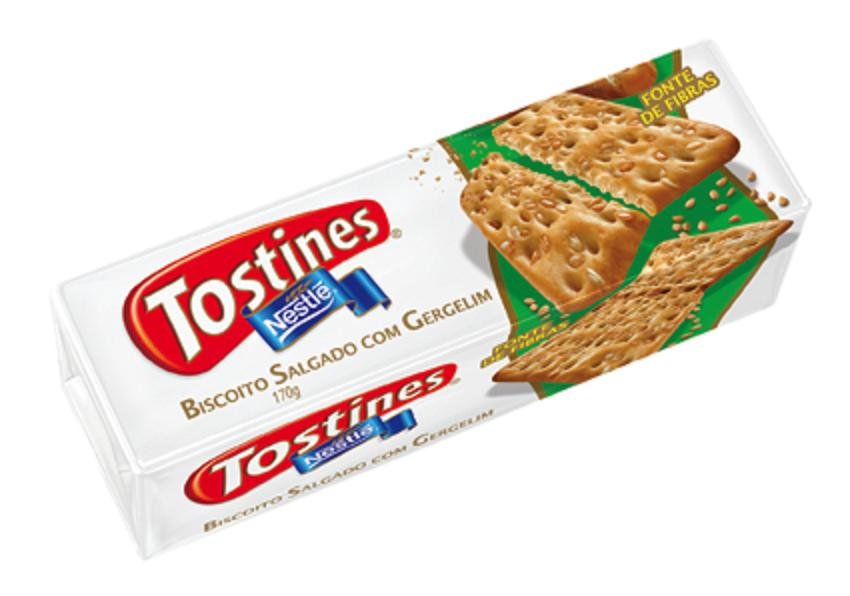
\includegraphics[scale=0.45]{tostines.jpg}
	\caption{Exemplo de objeto causador de Efeito Tostines}
	\label{fig-tostines}
\end{figure}

\blindtext[2]

\section[Conceito2]{Segundo Conceito}

\blindtext

\blindtext[2]

\blindtext
		

